%%%%%%%%%%%%%%%%%%%%%%%%%%%%%%%%%%%%%%%%%
% Jacobs Landscape Poster
% LaTeX Template
% Version 1.0 (29/03/13)
%
% Created by:
% Computational Physics and Biophysics Group, Jacobs University
% https://teamwork.jacobs-university.de:8443/confluence/display/CoPandBiG/LaTeX+Poster
% 
% Further modified by:
% Nathaniel Johnston (nathaniel@njohnston.ca)
%
% This template has been downloaded from:
% http://www.LaTeXTemplates.com
%
% License:
% CC BY-NC-SA 3.0 (http://creativecommons.org/licenses/by-nc-sa/3.0/)
%
%%%%%%%%%%%%%%%%%%%%%%%%%%%%%%%%%%%%%%%%%

%----------------------------------------------------------------------------------------
%	PACKAGES AND OTHER DOCUMENT CONFIGURATIONS
%----------------------------------------------------------------------------------------

\documentclass[final]{beamer}

\usepackage[scale=1.24]{beamerposter} % Use the beamerposter package for laying out the poster

\usetheme{confposter} % Use the confposter theme supplied with this template

\setbeamercolor{block title}{fg=ngreen,bg=white} % Colors of the block titles
\setbeamercolor{block body}{fg=black,bg=white} % Colors of the body of blocks
\setbeamercolor{block alerted title}{fg=white,bg=dblue!70} % Colors of the highlighted block titles
\setbeamercolor{block alerted body}{fg=black,bg=dblue!10} % Colors of the body of highlighted blocks
% Many more colors are available for use in beamerthemeconfposter.sty

%-----------------------------------------------------------
% Define the column widths and overall poster size
% To set effective sepwid, onecolwid and twocolwid values, first choose how many columns you want and how much separation you want between columns
% In this template, the separation width chosen is 0.024 of the paper width and a 4-column layout
% onecolwid should therefore be (1-(# of columns+1)*sepwid)/# of columns e.g. (1-(4+1)*0.024)/4 = 0.22
% Set twocolwid to be (2*onecolwid)+sepwid = 0.464
% Set threecolwid to be (3*onecolwid)+2*sepwid = 0.708

\newlength{\sepwid}
\newlength{\onecolwid}
\newlength{\twocolwid}
\newlength{\threecolwid}
\setlength{\paperwidth}{48in} % A0 width: 46.8in
\setlength{\paperheight}{36in} % A0 height: 33.1in
\setlength{\sepwid}{0.024\paperwidth} % Separation width (white space) between columns
\setlength{\onecolwid}{0.22\paperwidth} % Width of one column
\setlength{\twocolwid}{0.464\paperwidth} % Width of two columns
\setlength{\threecolwid}{0.708\paperwidth} % Width of three columns
\setlength{\topmargin}{-0.5in} % Reduce the top margin size
%-----------------------------------------------------------

\usepackage{graphicx}  % Required for including images

\usepackage{booktabs} % Top and bottom rules for tables

%----------------------------------------------------------------------------------------
%	TITLE SECTION 
%----------------------------------------------------------------------------------------

\title{Frequently Cited Passages Across Time: \\ New
Methods for Studying the Critical Reception of
Texts} % Poster title

\author{Jonathan Reeve, Sierra Eckert, Milan Terlunen} % Author(s)

\institute{Department of English and Comparative Literature, Columbia University} % Institution(s)

%----------------------------------------------------------------------------------------

\begin{document}

\addtobeamertemplate{block end}{}{\vspace*{2ex}} % White space under blocks
\addtobeamertemplate{block alerted end}{}{\vspace*{2ex}} % White space under highlighted (alert) blocks

\setlength{\belowcaptionskip}{2ex} % White space under figures
\setlength\belowdisplayshortskip{2ex} % White space under equations

\begin{frame}[t] % The whole poster is enclosed in one beamer frame

\begin{columns}[t] % The whole poster consists of three major columns, the second of which is split into two columns twice - the [t] option aligns each column's content to the top

\begin{column}{\sepwid}\end{column} % Empty spacer column

\begin{column}{\onecolwid} % The first column

%----------------------------------------------------------------------------------------
%	OBJECTIVES
%----------------------------------------------------------------------------------------

\begin{alertblock}{Research Questions}

We use text reuse detection to identify frequently cited passages from George Eliot's novel \emph{Middlemarch} in a corpus of over 4,000 critical articles (1950-2015) obtained from JSTOR that contain the word ``Middlemarch.'' We attempt to answer questions like: 

\begin{itemize}
\item What passages of the novel are critics most interested in quoting? How do these critical favorites change over time?  
\item Can we detect a life-cycle for certain passages which rise and fall in popularity over time?
\item What are the linguistic properties of quotations, as compared with non-quotations?
\item What makes us, as readers, choose to quote one passage instead of another? Can this be connected to major movements within the field (e.g. feminist criticism, deconstruction), institutional structures (eg. particular journals) or even to a specific critic?
\end{itemize}

\end{alertblock}

%----------------------------------------------------------------------------------------
%	INTRODUCTION
%----------------------------------------------------------------------------------------

\begin{block}{Methods}

We use a custom-built text reuse detection algorithm, text-matcher, that uses approximate text matching in a two-pass process to identify similar passages between texts. The first pass uses sequence matching to find a single matching trigram between the two texts. The algorithm then compares Levenshtein  distance ratios of boundary words.\\

\vspace{10mm}

We then visualize these results at different scales. First, we analyze this according to narrative position within the novel, (a heat map visualizing citations at the book and chapter level; a text browser showing sentence and paragraph level citations). Second, we analyze using corpus metadata. Finally, we examine the linguistic properties of the quotations themselves. These results reveal several striking patterns discussed in the following sections.  


\end{block}



%------------------------------------------------


%----------------------------------------------------------------------------------------

\end{column} % End of the first column

\begin{column}{\sepwid}\end{column} % Empty spacer column

\begin{column}{\twocolwid} % Begin a column which is two columns wide (column 2)

\begin{columns}[t,totalwidth=\twocolwid] % Split up the two columns wide column

\begin{column}{\onecolwid}\vspace{-.6in} % The first column within column 2 (column 2.1)

%----------------------------------------------------------------------------------------
%	MATERIALS
%----------------------------------------------------------------------------------------

\begin{block}{Frequently Quoted Chapters}

\begin{figure}
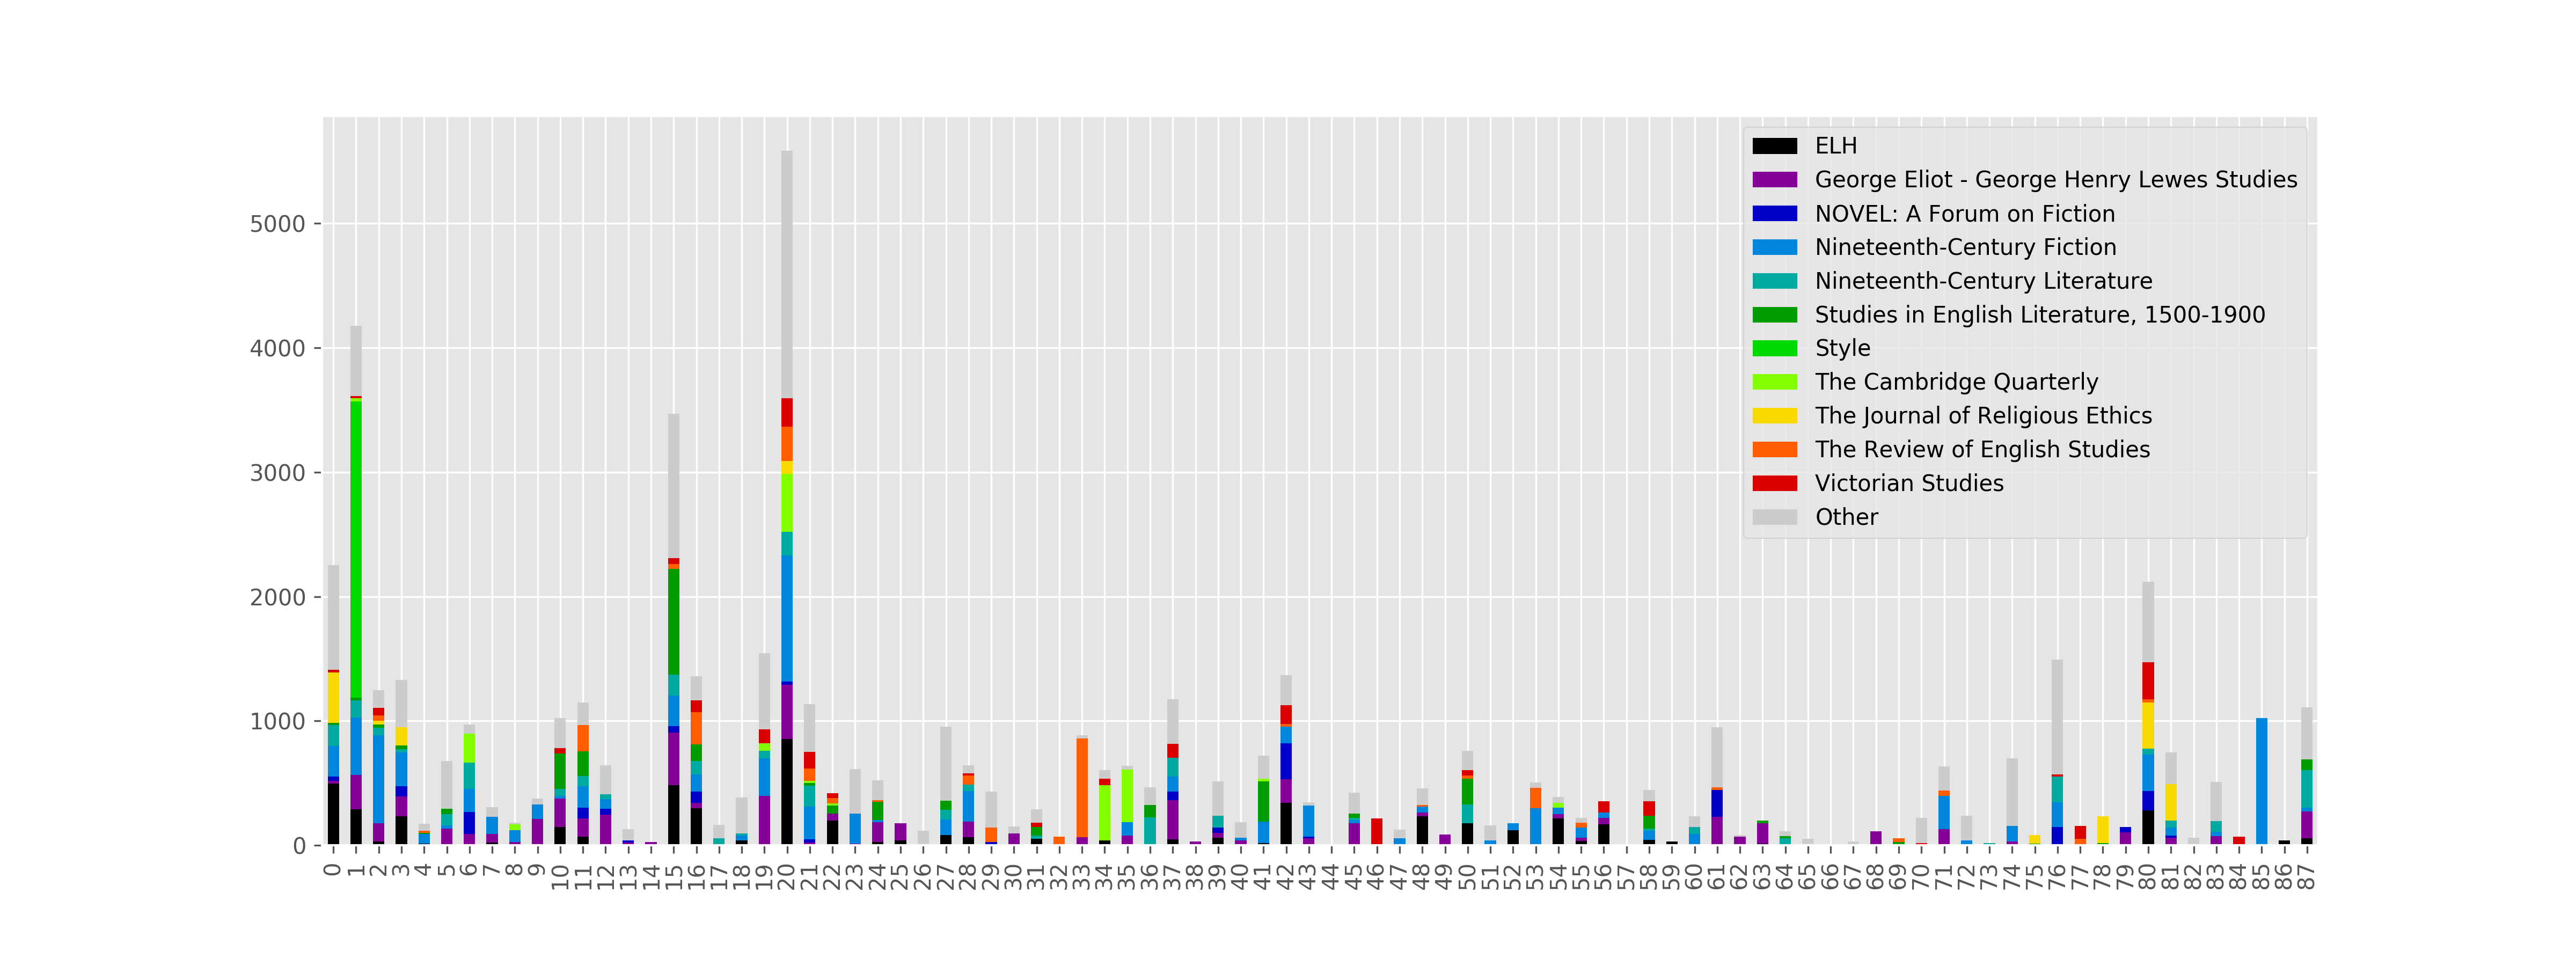
\includegraphics[width=0.9\linewidth]{synchronic-journals.png}
\caption{Quoted words by chapter, subdivided by journal.}
\end{figure}

Journals play a role in determining the relative number of citations of a given chapter, \emph{Style}, for instance, contributes heavily to the number of Chapter 1 citations.  Critical attention, across journals, tends to favor the first half of the novel.

\end{block}

%----------------------------------------------------------------------------------------

\end{column} % End of column 2.1

\begin{column}{\onecolwid}\vspace{-.6in} % The second column within column 2 (column 2.2)

%----------------------------------------------------------------------------------------
%	METHODS
%----------------------------------------------------------------------------------------

\begin{block}{Literary Critical Specialization}

Literary critics writing in the specialist journal \emph{George Eliot / George Henry Lewes Studies} quote different passages from their counterparts publishing in more generalist journals. A positive score here indicates a chapter is quoted more by specialists:  

\begin{figure}
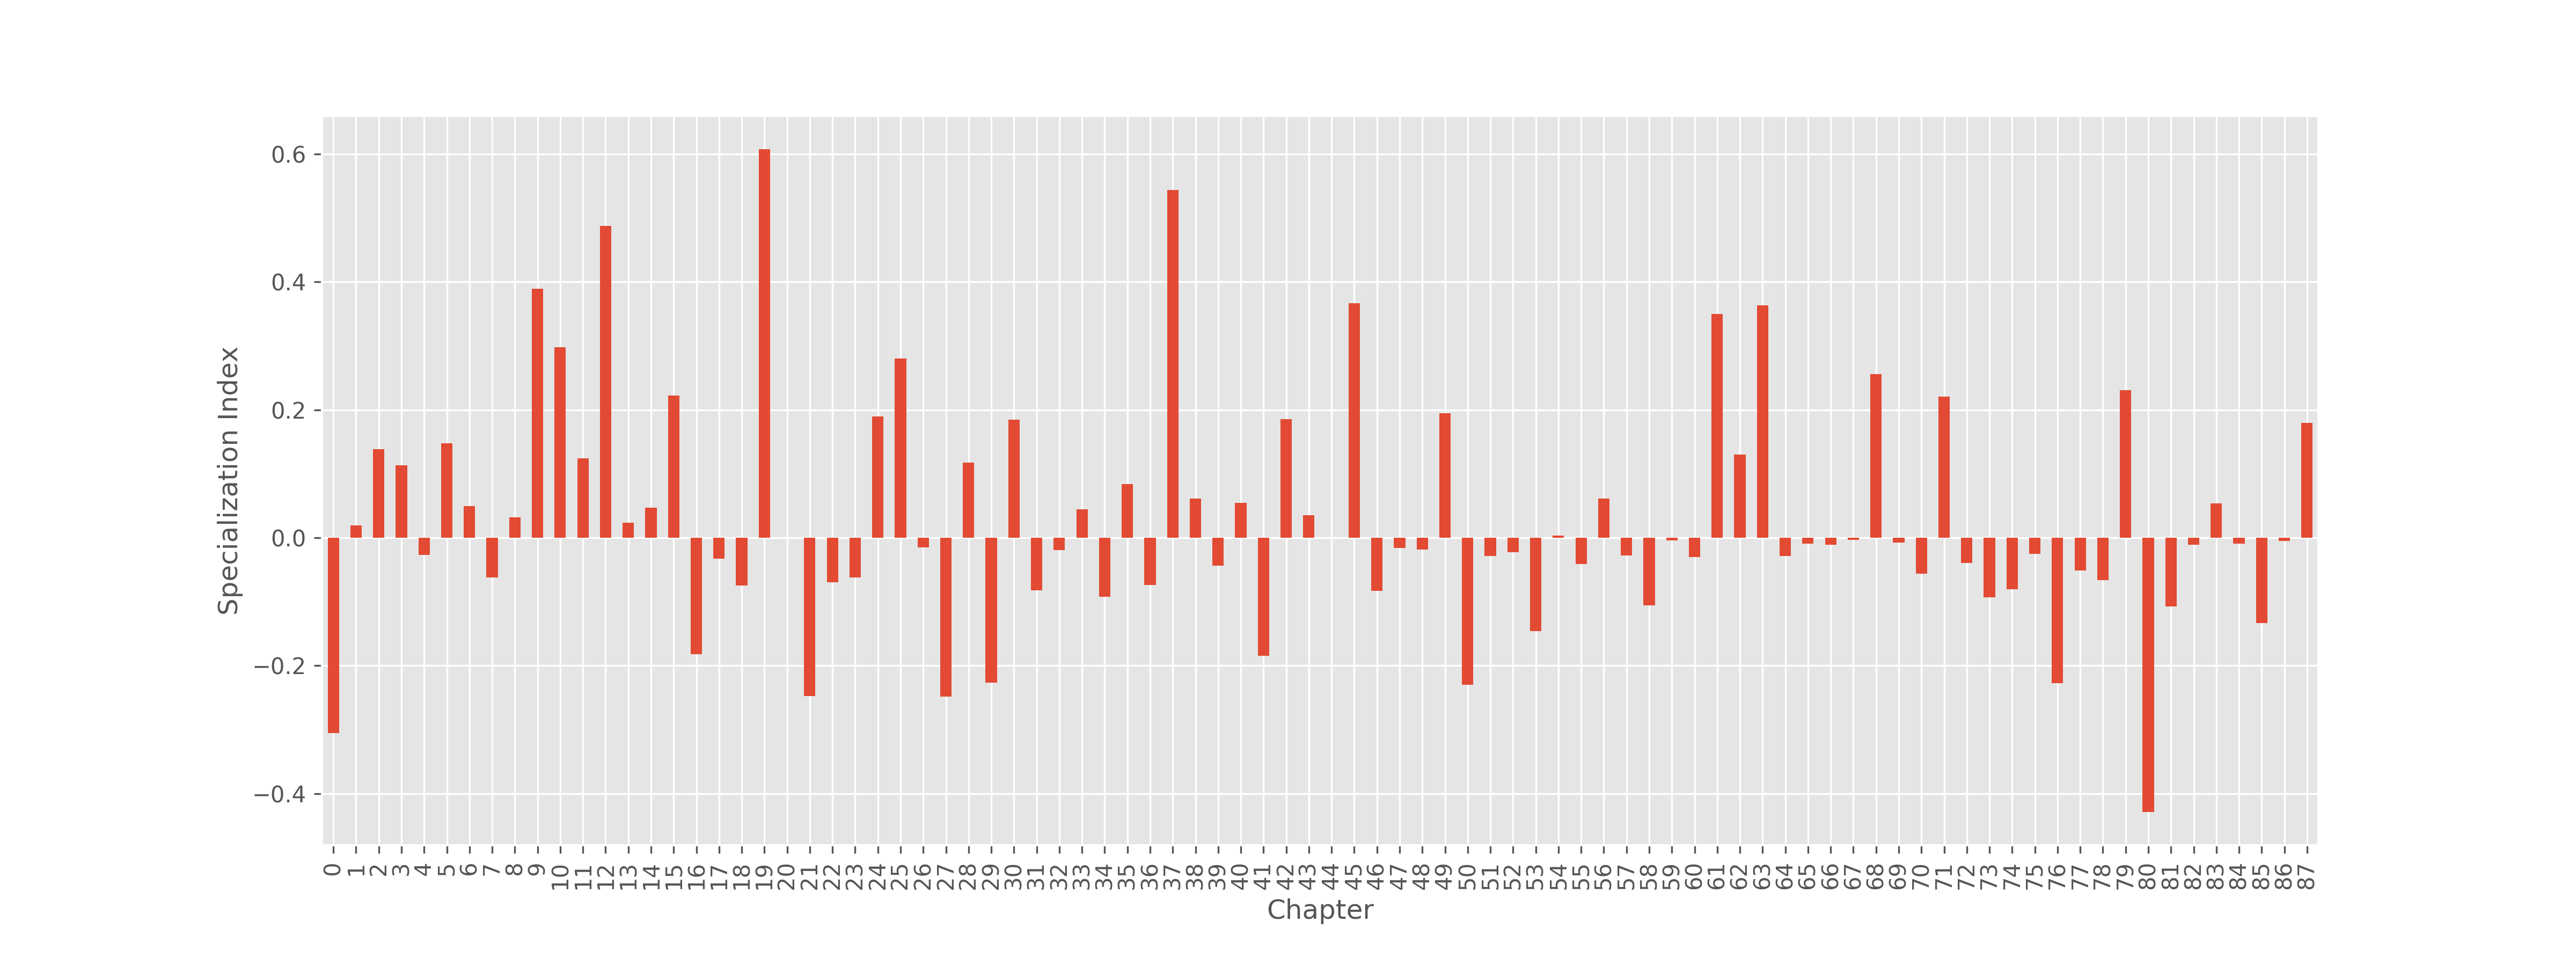
\includegraphics[width=0.9\linewidth]{specialization.png}
\caption{Chapters quoted, specialists vs. non-specialists.}
\end{figure}


\end{block}

%----------------------------------------------------------------------------------------

\end{column} % End of column 2.2

\end{columns} % End of the split of column 2 - any content after this will now take up 2 columns width

%----------------------------------------------------------------------------------------
%	IMPORTANT RESULT
%----------------------------------------------------------------------------------------

\begin{alertblock}{\emph{Middlemarch}: Shifts in Critical Attention over Time}

Viewed diachronically, trends arise in critical quotations of the novel. Critics' favorite chapters to excerpt shift from Chapter 81 in the 1950s to Chapter 20 in the 60s-70s, and to Chapter 15 in the 80s-90s. 

\begin{figure}
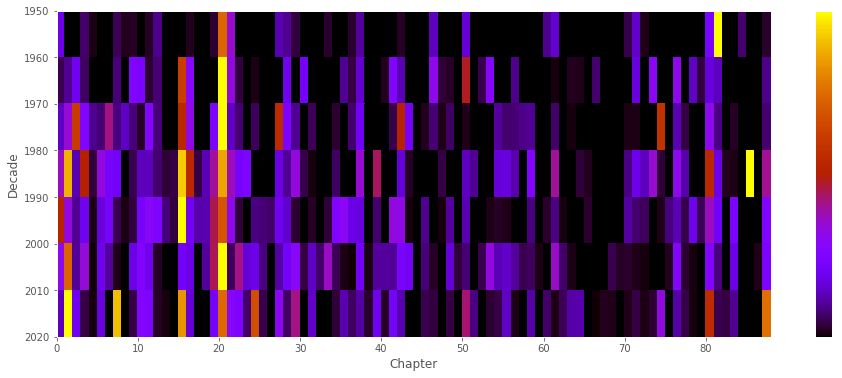
\includegraphics[width=0.8\linewidth]{diachronic.png}
\end{figure}

\end{alertblock} 

%----------------------------------------------------------------------------------------


\begin{block}{From the Critical Heatmap Edition: Most Quoted Passage}

\begin{figure}
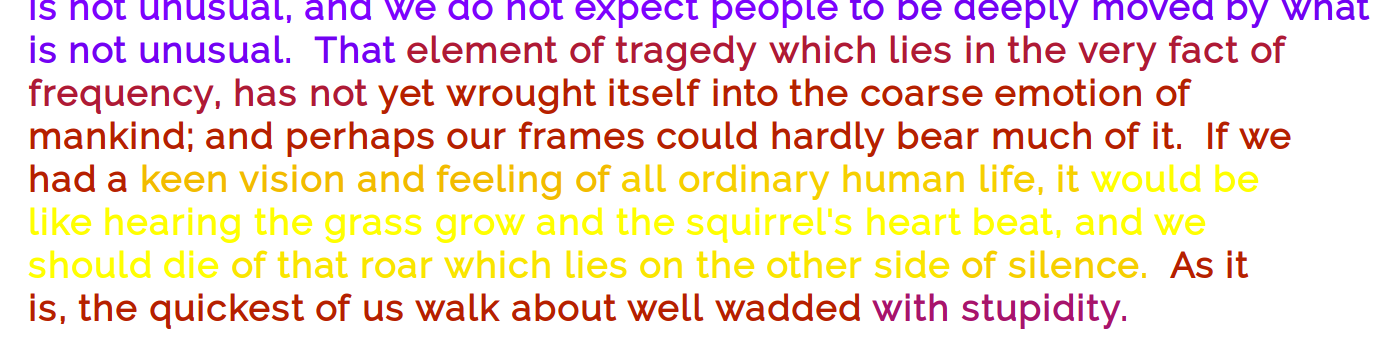
\includegraphics[width=0.7\linewidth]{most-quoted.png}
\end{figure}
\end{block} 

\end{column} % End of the second column

\begin{column}{\sepwid}\end{column} % Empty spacer column

\begin{column}{\onecolwid} % The third column

%----------------------------------------------------------------------------------------
%	CONCLUSION
%----------------------------------------------------------------------------------------

\begin{block}{Properties of Quotations}

Figure 5 shows characteristic parts of speech of quotations (positive), and non-quotations (negative). 

\begin{figure}
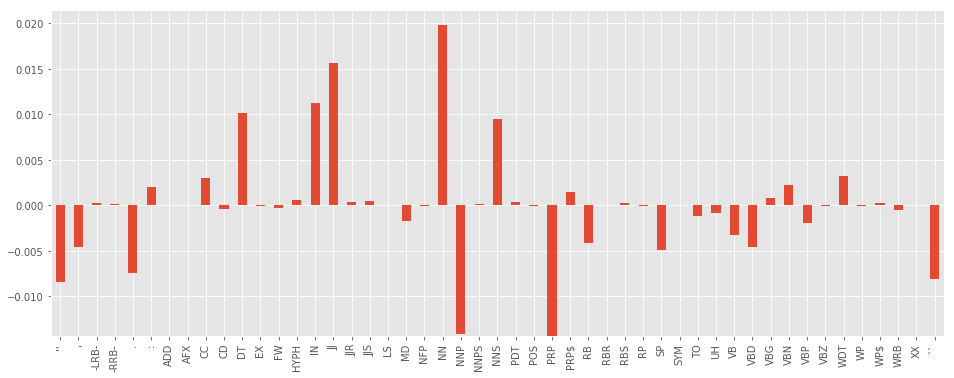
\includegraphics[width=0.9\linewidth]{pos-tags.png}
\caption{Distinctive parts of speech of quotations}
\end{figure}

Table 1 shows most distinctive words of non-quotes (negative, above), and quotes (positive, below): 

\begin{table}
\vspace{2ex}
\begin{tabular}{l l}
\toprule
\textbf{Word} & \textbf{Freq. Diff.} \\
\midrule
say           &  -0.006397 \\
lydgate       &  -0.004499 \\
mr.           &  -0.003395 \\
bulstrode     &  -0.002948 \\
fred          &  -0.002781 \\
rosamond      &  -0.002616 \\
\midrule
eye          &   0.001024 \\
live         &   0.001042 \\
consciousness &   0.001054 \\
great        &   0.001080 \\
new          &   0.001134 \\
woman        &   0.001154 \\
world        &   0.001883 \\
light        &   0.002183 \\
life         &   0.002417 \\
\bottomrule
\end{tabular}
\caption{(Non-)Distinctive words of quotations}
\end{table}

\end{block}

%----------------------------------------------------------------------------------------
%	ADDITIONAL INFORMATION
%----------------------------------------------------------------------------------------

\begin{block}{Links and Contacts}

\begin{itemize}
\item Project page: github.com/lit-mod-viz/middlemarch-critical-histories
\item Jonathan Reeve: jonathan.reeve@columbia.edu
\item Sierra Eckert: sierra.eckert@columbia.edu
\item Milan Terlunen: m.terlunen@columbia.edu 
\end{itemize}

\end{block}

%----------------------------------------------------------------------------------------

\end{column} % End of the third column

\end{columns} % End of all the columns in the poster

\end{frame} % End of the enclosing frame

\end{document}
